\documentclass{article}
\usepackage{graphicx}
\usepackage{xcolor}
\usepackage{multirow}
\usepackage{subcaption}
\usepackage[utf8]{inputenc}



\usepackage[export]{adjustbox}

\usepackage{amsmath}
\usepackage{amsfonts}
\usepackage{amssymb}
\usepackage[version=4]{mhchem}
\usepackage{stmaryrd}
\usepackage{hyperref}
\hypersetup{colorlinks=true, linkcolor=blue, filecolor=magenta, urlcolor=cyan,}
\urlstyle{same}

\date{September 10, 2023}
\begin{document}

\begin{figure}
\centering

\includegraphics[width=0.9\linewidth, keepaspectratio]{logo}
\end{figure}
\author{EE20B149\\Varun M}
\title{\textbf{BT6270: Computational Neuroscience\\Assignment 1\\}}
\maketitle
\newpage
\section{Introduction}
The Hodgkin-Huxley model explains how the dynamics of ion channels (Na+, K+ etc) contribute to the generation of an Action Potential in a neuron.\\
An Action Potential is a sharp voltage spike elicited by stimulating a neuron with a current that exceeds a certain threshold value. The current amplitude is increased gradually, at a threshold amplitude, the voltage response does not increase proportionally. \\
It shows a sharp, disproportionate increase.\\ Once the membrane voltage reaches a threshold value, it increase further rapidly to maximum value and drops again rapidly to a value that is less than resting value, before returning to the baseline value after a delay.
\begin{figure}[h]
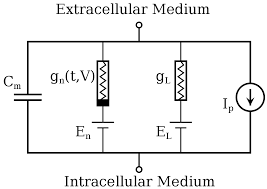
\includegraphics[width=8cm]{hh.png}
\caption{Hodgkin-Huxley model circuit}
\end{figure}
\section{Neural Firing Frequencies and Thresholding}
\subsection{Threshold Values of External Current}
The Threshold Currents are as follows:
\begin{itemize}
    \item I1 = 0.023 $\mu A/ mm^2$
    \vspace{-3mm}
    \item I2 = 0.0615 $\mu A/ mm^2$
    \vspace{-3mm}
    \item I3 = 0.458 $\mu A/ mm^2$
\end{itemize}
These values were obtained by setting the sampling interval to 0.001 between [0,0.6]. The value of 0.6 is chosen after hit and trial on the MATLAB code and analyzing the Voltage vs Time graph. All the I1, I2 and I3 values don't exceed more than 0.6.
\subsection{Assumptions}
Assumptions for the plot are as follows:
\begin{itemize}
    \item A peak must exceed a threshold voltage of \textbf{5 mV} in order to be classified as an action potential.
    \item I1 is calculated at the initial non-zero value of the number of Voltage Peaks.
    \item I2 is calculated at the input current value where the following current instant has \textbf{3} or more voltage peaks exceeding \textbf{5 mV}.
    \item I3 is calculated as the input current value at which there are \textbf{7} or more voltage peaks above 5 mV in the next current instant.
\end{itemize}
\subsection{Plots}
\subsubsection{Frequency vs Input current}
\begin{itemize}
    \item As we can see in the obtained plots, we start getting periodic action potentials from 0.0224$\mu$A to 0.5432$\mu$A.\\
    \item Thus we can obtain a frequency vs input current plot for the same. The frequency will be zero initially till 0.0224$\mu$A.\\
    \item After that we get a frequency value at 0.0224$\mu$A and it increases till the input current in increased till 0.5432$\mu$A.\\
    \item After 0.5432$\mu$A again we get zero frequency as we do not have action potentials.
\end{itemize}
\newpage
\subsubsection{Region 1}
\begin{figure}[h]
    \centering
    \begin{subfigure}[b]{0.45\textwidth}
        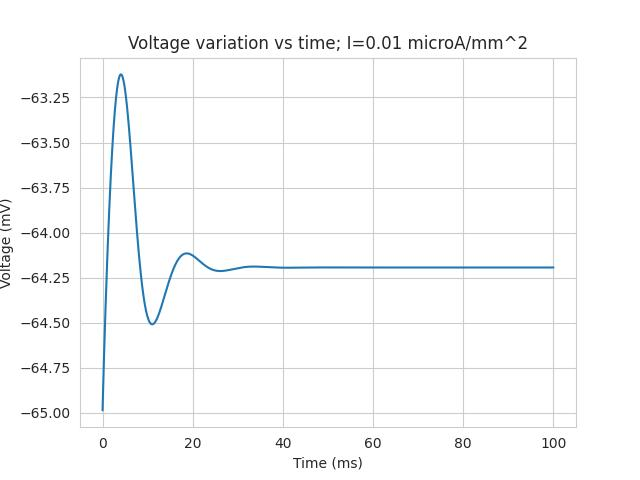
\includegraphics[width=1.5\textwidth]{1.jpg}
        \caption{Plot of Voltage vs Time for I=0.01$\mu$A}
        \label{fig:IOU1}
    \end{subfigure}
    
     %add desired spacing between images, e. g. ~, \quad, \qquad, \hfill etc. 
      %(or a blank line to force the subfigure onto a new line)
    \begin{subfigure}[b]{0.45\textwidth}
        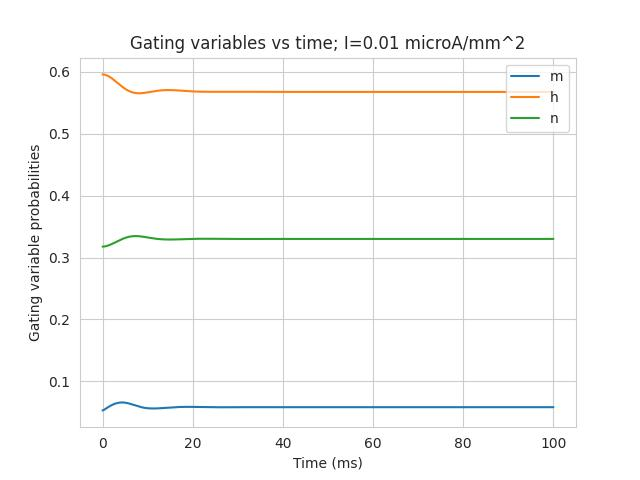
\includegraphics[width=1.5\textwidth]{2.jpg}
        \caption{Plot of gating variables for I=0.01$\mu$A}
        \label{fig:IO2}
    \end{subfigure}
    %add desired spacing between images, e. g. ~, \quad, \qquad, \hfill etc. 
    %(or a blank line to force the subfigure onto a new line)
    \begin{subfigure}[b]{0.45\textwidth}
        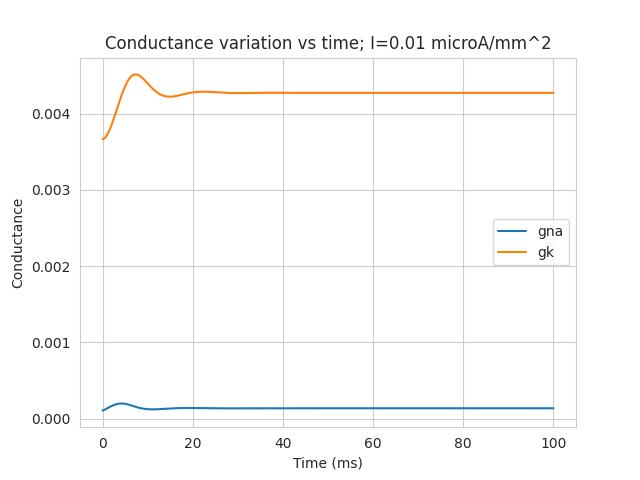
\includegraphics[width=1.5\textwidth]{3.jpg}
        \caption{Plot of conductances for I=0.01$\mu$A}
        \label{fig:IO2}
    \end{subfigure}
\end{figure}
\newpage
\subsubsection{Region 2}

\begin{figure}[h]
    \centering
    \begin{subfigure}[h]{0.45\textwidth}
        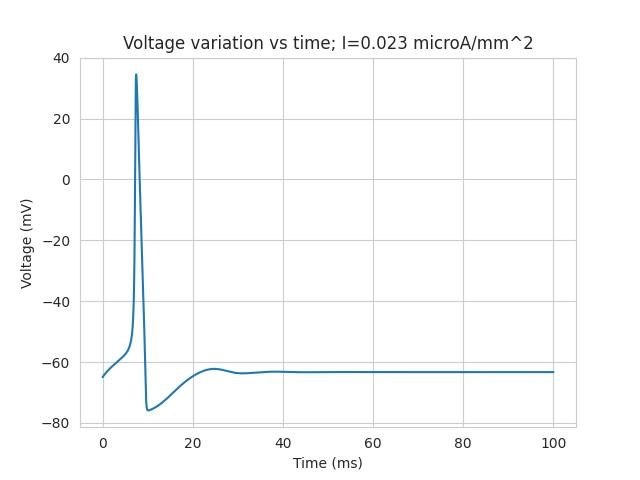
\includegraphics[width=1.5\textwidth]{4.jpg}
        \caption{Plot of Voltage vs Time for I=0.023$\mu$A}
        \label{fig:IOU1}
    \end{subfigure}
    
     %add desired spacing between images, e. g. ~, \quad, \qquad, \hfill etc. 
      %(or a blank line to force the subfigure onto a new line)
    \begin{subfigure}[b]{0.45\textwidth}
        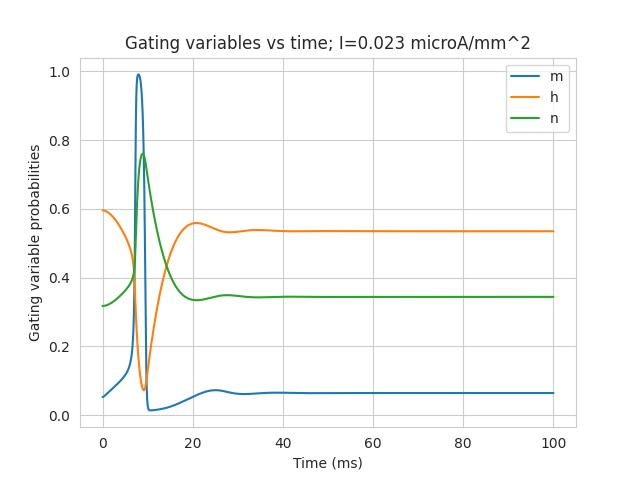
\includegraphics[width=1.5\textwidth]{5.jpg}
        \caption{Plot of gating variables for I=0.023$\mu$A}
        \label{fig:IO2}
    \end{subfigure}
    %add desired spacing between images, e. g. ~, \quad, \qquad, \hfill etc. 
    %(or a blank line to force the subfigure onto a new line)
    \begin{subfigure}[b]{0.45\textwidth}
        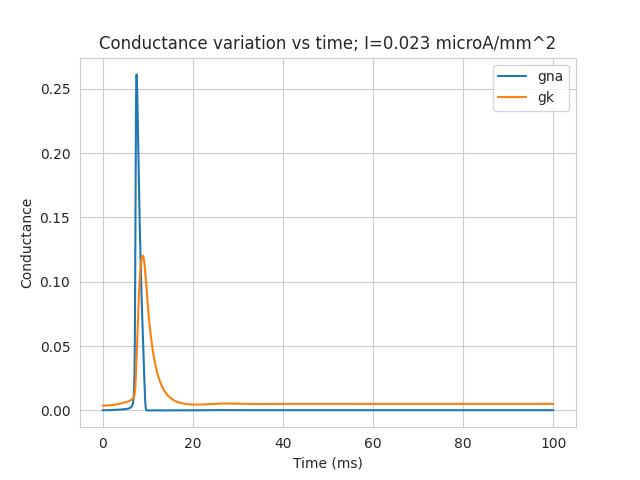
\includegraphics[width=1.5\textwidth]{6.jpg}
        \caption{Plot of conductances for I=0.023$\mu$A}
        \label{fig:IO2}
    \end{subfigure}
\end{figure}
\newpage
\subsubsection{Region 3}

\begin{figure}[h]
    \centering
    \begin{subfigure}[b]{0.45\textwidth}
        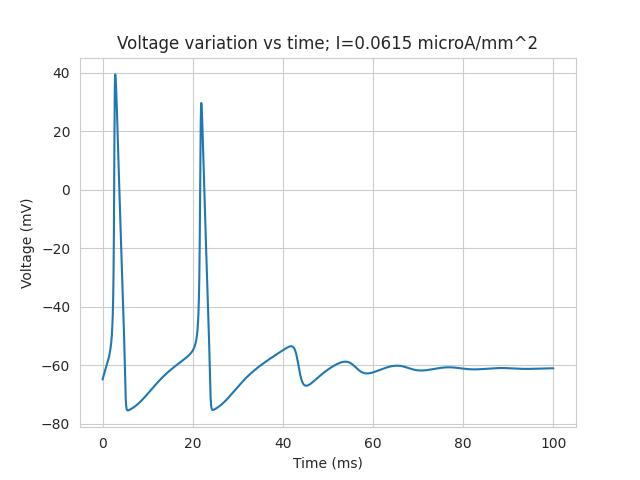
\includegraphics[width=1.5\textwidth]{7.jpg}
        \caption{Plot of Voltage vs Time for I=0.0615$\mu$A}
        \label{fig:IOU1}
    \end{subfigure}
    
     %add desired spacing between images, e. g. ~, \quad, \qquad, \hfill etc. 
      %(or a blank line to force the subfigure onto a new line)
    \begin{subfigure}[b]{0.45\textwidth}
        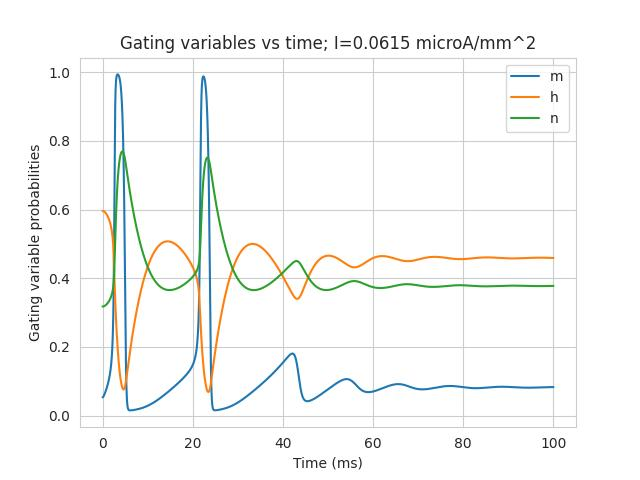
\includegraphics[width=1.5\textwidth]{8.jpg}
        \caption{Plot of gating variables for I=0.0.0615$\mu$A}
        \label{fig:IO2}
    \end{subfigure}
    %add desired spacing between images, e. g. ~, \quad, \qquad, \hfill etc. 
    %(or a blank line to force the subfigure onto a new line)
    \begin{subfigure}[b]{0.45\textwidth}
        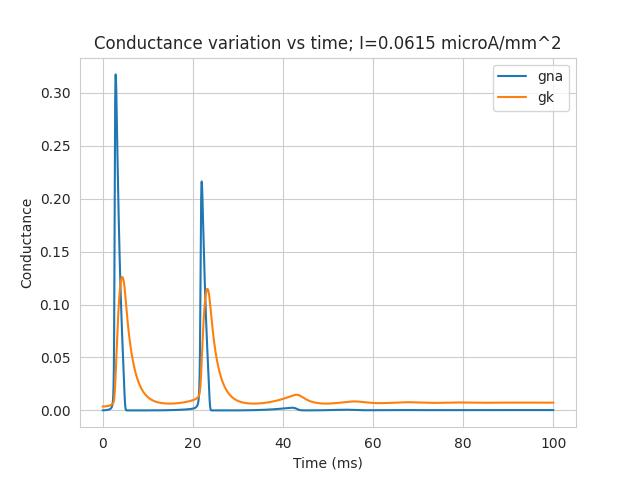
\includegraphics[width=1.5\textwidth]{9.jpg}
        \caption{Plot of conductances for I=0.0615$\mu$A}
        \label{fig:IO2}
    \end{subfigure}
\end{figure}
\newpage
\subsubsection{Region 4}

\begin{figure}[h]
    \centering
    \begin{subfigure}[b]{0.45\textwidth}
        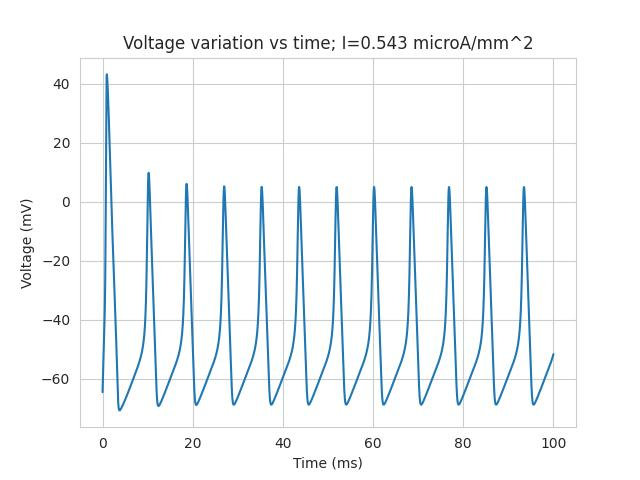
\includegraphics[width=1.5\textwidth]{10.jpg}
        \caption{Plot of Voltage vs Time for I=0.543$\mu$A}
        \label{fig:IOU1}
    \end{subfigure}
    
     %add desired spacing between images, e. g. ~, \quad, \qquad, \hfill etc. 
      %(or a blank line to force the subfigure onto a new line)
    \begin{subfigure}[b]{0.45\textwidth}
        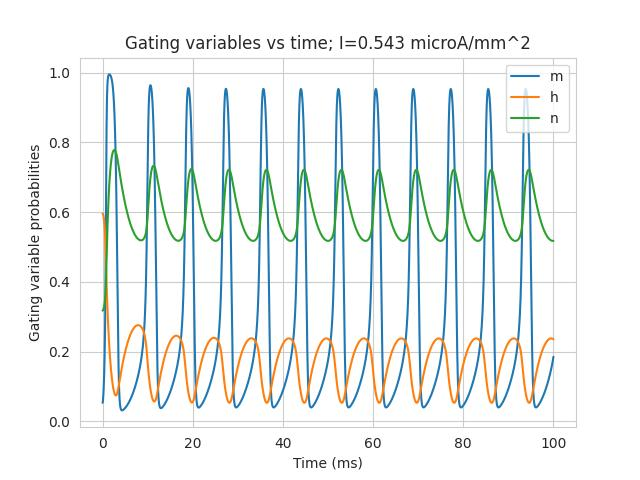
\includegraphics[width=1.5\textwidth]{11.jpg}
        \caption{Plot of gating variables for I=0.543$\mu$A}
        \label{fig:IO2}
    \end{subfigure}
    %add desired spacing between images, e. g. ~, \quad, \qquad, \hfill etc. 
    %(or a blank line to force the subfigure onto a new line)
    \begin{subfigure}[b]{0.45\textwidth}
        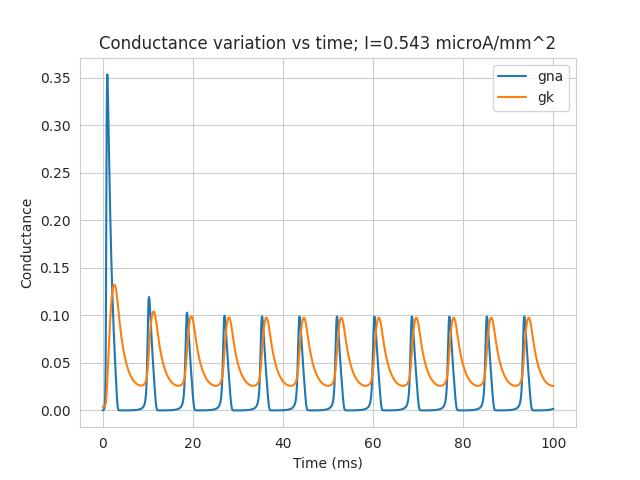
\includegraphics[width=1.5\textwidth]{12.jpg}
        \caption{Plot of conductances for I=0.543$\mu$A}
        \label{fig:IO2}
    \end{subfigure}
\end{figure}
\newpage
\subsubsection{Region 5}

\begin{figure}[h]
    \centering
    \begin{subfigure}[b]{0.45\textwidth}
        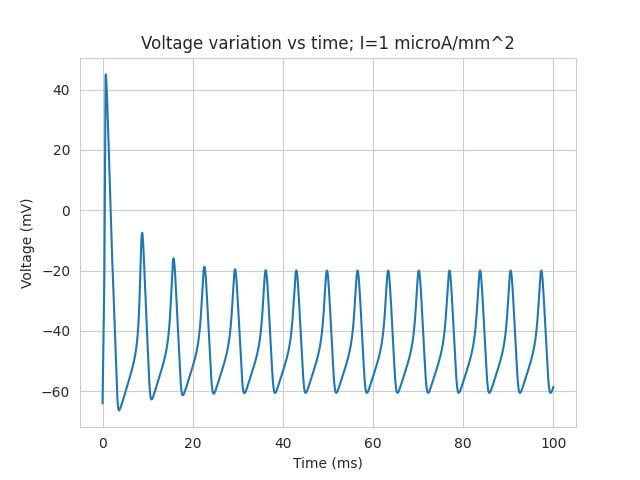
\includegraphics[width=1.5\textwidth]{13.jpg}
        \caption{Plot of Voltage vs Time for I=1$\mu$A}
        \label{fig:IOU1}
    \end{subfigure}
    
     %add desired spacing between images, e. g. ~, \quad, \qquad, \hfill etc. 
      %(or a blank line to force the subfigure onto a new line)
    \begin{subfigure}[b]{0.45\textwidth}
        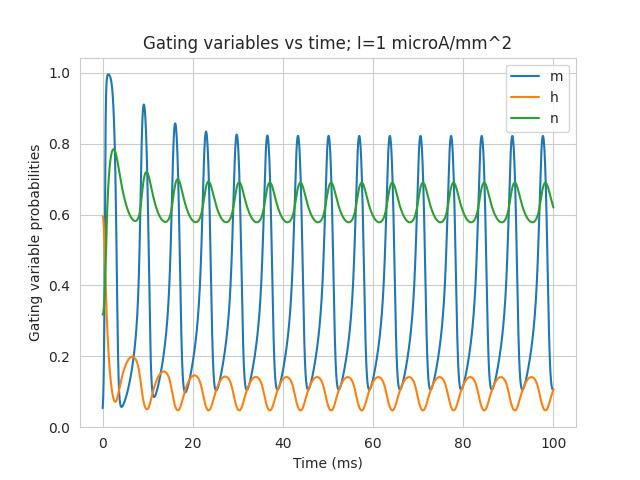
\includegraphics[width=1.5\textwidth]{14.jpg}
        \caption{Plot of gating variables for I=1$\mu$A}
        \label{fig:IO2}
    \end{subfigure}
    %add desired spacing between images, e. g. ~, \quad, \qquad, \hfill etc. 
    %(or a blank line to force the subfigure onto a new line)
    \begin{subfigure}[b]{0.45\textwidth}
        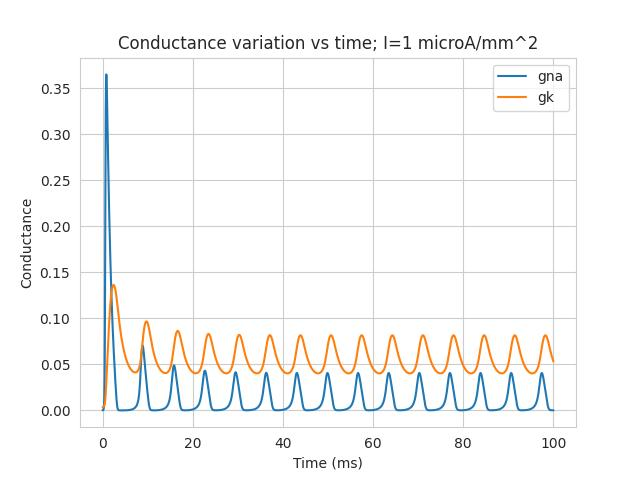
\includegraphics[width=1.5\textwidth]{15.jpg}
        \caption{Plot of conductances for I=1$\mu$A}
        \label{fig:IO2}
    \end{subfigure}
\end{figure}




\newpage
\section{Frequency vs Input current plot}
We have zero frequency before and after Region 3.

 \begin{figure}[h]
 \centering
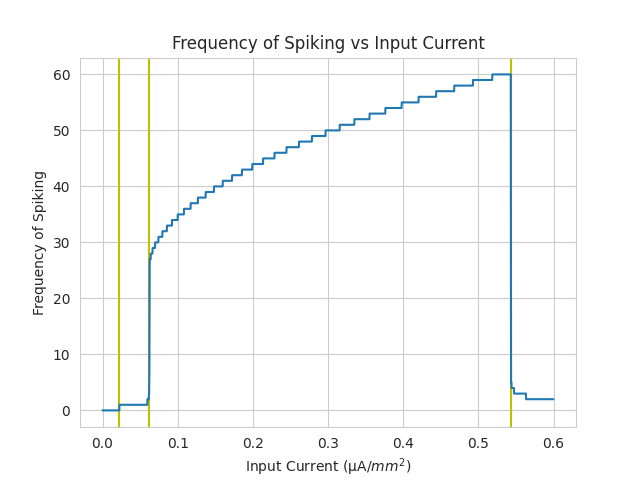
\includegraphics[width=10cm]{freq.png}
\caption{Frequency vs Input current plot}

\end{figure}




%``I always thought something was fundamentally wrong with the universe'' \citep{adams1995hitchhiker}

\bibliographystyle{plain}
\end{document}